\documentclass[11pt]{book}
%\usepackage[subpreambles=true]{standalone}
\usepackage[spanish]{babel}
\usepackage{comfortaa}
\usepackage[T1]{fontenc}
\usepackage[utf8]{inputenc}
\usepackage[
letterpaper,
left=1in, 
right=1in, 
top=1in,
bottom=1in,
headheight=10mm,% Set \headheight to 10mm
]{geometry} % Custom margins
\usepackage{float}
\usepackage[colorlinks = true, linkcolor = colorrds]{hyperref}
\usepackage{bookmark}
\usepackage{fancyhdr}
\usepackage{color, colortbl}
\usepackage[dvipsnames,table]{xcolor} % Required for custom color
\usepackage{graphicx}
\usepackage{tabularx}
\usepackage{multicol,multirow}
\usepackage{newclude}
\usepackage{tabto}
\usepackage{remreset}
\usepackage[inline]{enumitem}
\usepackage{xparse}
\usepackage{wrapfig}
\usepackage{caption,capt-of}
\usepackage{amssymb,amsmath}
\usepackage{tikz}
\usepackage{subfiles}
\usepackage{etoolbox}
\usepackage{pdflscape}
\usepackage[explicit]{titlesec}
\usepackage{subfiles} % Best loaded last in the preamble
\input{insbox}
\makeatletter
\@removefromreset{section}{chapter}
\makeatother
\addto\captionsspanish{\renewcommand{\chaptername}{Unidad}}
\renewcommand{\thechapter}{\arabic{chapter}}
\renewcommand{\thesection}{S\arabic{section}}
\renewcommand{\thesubsection}{L\arabic{subsection}}
\newcommand*\chapterlabel{}
\titleformat{\chapter}
{\gdef\chapterlabel{}
    \comfortaa\Huge\bfseries
}
{\gdef\chapterlabel{\chaptername \ \thechapter}}{0pt}
{\begin{tikzpicture}[remember picture,overlay]
        \node[yshift=-2cm] at (current page.north west)
        {\begin{tikzpicture}[remember picture, overlay]
                \draw[draw=none,fill=teal] (0,0) rectangle
                (\paperwidth,2cm);
                \node[anchor=east,xshift=.9\paperwidth,rectangle,
                    rounded corners=5pt,inner xsep=20pt,inner ysep=5pt,
                    blur shadow={shadow blur steps=50,shadow blur extra rounding=5pt},
                    fill=brown]
                {\color{CadetBlue!20}\textbf{\chapterlabel#1}};
            \end{tikzpicture}
        };
    \end{tikzpicture}
}
\titlespacing*{\chapter}{0pt}{50pt}{-60pt}

\makeatletter
\@removefromreset{section}{chapter}
\makeatother
\addto\captionsspanish{\renewcommand{\chaptername}{Unidad}}
\renewcommand{\thechapter}{\arabic{chapter}}
\renewcommand{\thesection}{S\arabic{section}}
\renewcommand{\thesubsection}{L\arabic{subsection}}
\newcommand*\sectionlabel{}
\titleformat{\section}
{\gdef\sectionlabel{}
    \comfortaa\large\bfseries
}
{\gdef\sectionlabel{\thesection \ }}{0pt}
{\begin{tikzpicture}[remember picture,overlay]
        \node[yshift=-1.5cm] at (current page.north west)
        {\begin{tikzpicture}[remember picture, overlay]
                \draw[draw=none,fill=colorrds!30,
                    %shade,
                    rounded corners=5pt,
                    blur shadow={shadow blur steps=10,shadow blur extra rounding=10pt},
                    xshift=5mm,
                ] (0,0) rectangle
                (\paperwidth-10mm,2cm);
                \node[
                    anchor=west,
                    xshift=0.1\paperwidth,
                    rectangle,
                    %shade,
                    rounded corners=5pt,
                    inner sep=8pt,
                    fill=olive!50,
                    %drop shadow={fill=black, opacity=1},
                ]
                {\color{colorrds}\sectionlabel#1};
                % \node[anchor=east,xshift=.9\paperwidth,rectangle,
                %     rounded corners=10pt,inner sep=11pt,
                %     fill=blue!35]
                % {\color{green}\sectionlabel};
            \end{tikzpicture}
        };
    \end{tikzpicture}
}
\titlespacing*{\section}{0pt}{50pt}{0pt}
\usepackage[many]{tcolorbox}
% \usepackage{mathspec} 			    % for FONTS
% \usepackage{setspace}               % for LINE SPACING
% \setmainfont{Noto Sans}[
%     Kerning = On,
%     Mapping = tex-text,
%     Numbers = Uppercase,
%     BoldFont = Noto Sans SemiBold
% ]                           % setting the font as Noto Sans
% \setlength\parindent{0pt}   % killing indentation for all the text
% \setstretch{1.3}            % setting line spacing to 1.3
% \setlength\columnsep{0.25in} % setting length of column separator
% \pagestyle{empty}           % setting pagestyle to be empty


\definecolor{main}{HTML}{5989cf}    % setting main color to be used
\definecolor{sub}{HTML}{cde4ff}     % setting sub color to be used

\tcbset{
    sharp corners,
    colback = white,
    before skip = 0.2cm,    % add extra space before the box
    after skip = 0.5cm      % add extra space after the box
}                           % setting global options for tcolorbox


\newtcolorbox{bA}{
    %sharpish corners, % b
    enhanced,
    %colback = sub, % background color
    boxrule = 0.2pt,  % no borders
    %borderline = {1pt}{1pt}{black!35}, % add "dashed" for dashed line
    %fontupper = \bf\color{black}, % font color
    %colframe = main % frame color
    rounded corners,
    %arc = 5pt,   % corners roundness
    fuzzy shadow = {2pt}{-4pt}{-1pt}{1pt}{black!35}, % {xshift}{yshift}{offset}{step}{options} 
    %toprule = 3pt, % top rule weight
    %bottomrule = 3pt % bottom rule weight
}
% You can copy any following box you like to your code.
\newtcolorbox{boxA}{
    fontupper = \bf,
    boxrule = 1.5pt,
    colframe = black % frame color
}

\newtcolorbox{boxB}{
    fontupper = \bf\color{main}, % font color
    boxrule = 1.5pt,
    colframe = main,
    rounded corners,
    arc = 5pt   % corners roundness
}

\newtcolorbox{boxC}{
    colback = sub, % background color
    boxrule = 0pt  % no borders
}

\newtcolorbox{boxD}{
    colback = sub,
    colframe = main,
    boxrule = 0pt,
    toprule = 3pt, % top rule weight
    bottomrule = 3pt % bottom rule weight
}

\newtcolorbox{boxE}{
    enhanced, % for a fancier setting,
    boxrule = 0pt, % clearing the default rule
    borderline = {0.75pt}{0pt}{main}, % outer line
    borderline = {0.75pt}{2pt}{sub} % inner line
}

\newtcolorbox{boxF}{
    colback = sub,
    enhanced,
    boxrule = 1.5pt,
    colframe = white, % making the base for dash line
    borderline = {1.5pt}{0pt}{main, dashed} % add "dashed" for dashed line
}

\newtcolorbox{boxG}{
    enhanced,
    boxrule = 0pt,
    colback = sub,
    borderline west = {1pt}{0pt}{main},
    borderline west = {0.75pt}{2pt}{main},
    borderline east = {1pt}{0pt}{main},
    borderline east = {0.75pt}{2pt}{main}
}

\newtcolorbox{boxH}{
    colback = colorrds!10,
    colframe = colorrds,
    boxrule = 0pt,
    leftrule = 6pt % left rule weight
}

\newtcolorbox{boxI}{
    colback = sub,
    colframe = main,
    boxrule = 0pt,
    toprule = 6pt % top rule weight
}

\newtcolorbox{boxJ}{
    sharpish corners, % better drop shadow
    colback = sub,
    colframe = main,
    boxrule = 0pt,
    toprule = 4.5pt, % top rule weight
    enhanced,
    fuzzy shadow = {0pt}{-2pt}{-0.5pt}{0.5pt}{black!35} % {xshift}{yshift}{offset}{step}{options} 
}

\newtcolorbox{boxK}{
    sharpish corners, % better drop shadow
    boxrule = 0pt,
    toprule = 4.5pt, % top rule weight
    enhanced,
    fuzzy shadow = {0pt}{-4pt}{-1pt}{1pt}{black!35} % {xshift}{yshift}{offset}{step}{options} 
}

\newtcolorbox{boxL}{
    fontupper = \color{main},
    rounded corners,
    arc = 6pt,
    colback = sub,
    colframe = main!50,
    boxrule = 0pt,
    bottomrule = 4.5pt
}

\newtcolorbox{boxM}{
    fontupper = \color{white},
    rounded corners,
    arc = 6pt,
    colback = main!80,
    colframe = main,
    boxrule = 0pt,
    bottomrule = 4.5pt,
    enhanced,
    fuzzy shadow = {0pt}{-3pt}{-0.5pt}{0.5pt}{black!35}
}
\decimalpoint
%\captionsetup{width=.45\textwidth}
\setlength{\parindent}{0pt}
\graphicspath{{./Images}} %Setting the graphicspath
\definecolor{colorrds}{HTML}{0060A0} % Custom colour
%%% Headings and footer
\renewcommand\spanishtablename{Tabla}
\cfoot{\thepage}
\renewcommand{\headrulewidth}{0.2pt}
\renewcommand{\footrulewidth}{0.2pt}
%%%
\usetikzlibrary{
  arrows,
  positioning,
  matrix,
  calc,
  decorations.pathreplacing,
  decorations.pathmorphing,
  decorations.markings,
  decorations.text,
  shapes.symbols,
  backgrounds,
  shadows.blur,
  trees,
  fit,
  snakes,
  patterns,
  mindmap,
  intersections,
  calendar,
  plotmarks,
  spy,
  tikzmark}

%%%% APRENDISAJES TEXTBOX
\tikzset{
  abstractbox/.style={
    draw=black, fill=white, rectangle, 
    inner sep=15pt, style=rounded corners,
    drop shadow={fill=black, opacity=1}
  },
  abstracttitle/.style={fill=white}
}
\newcommand{\boxabstract}[2][fill=white]{
  \begin{tikzpicture}
    \node [abstractbox, #1] (box)
    {\begin{minipage}{0.9\linewidth}
        \setlength{\parindent}{0mm} % Indentar.
        \normalfont #2
      \end{minipage}};
    \node[abstracttitle, right=5pt] at (box.north west) {\textbf{Aprendizajes esperados:}};
    \node[draw=none, fit=(box)] {};
  \end{tikzpicture}
}%
%%%%%%%%%%%%%%%%%%%%%%%%
%\renewcommand{\labelenumi}{\mbox{\arabic{enumi}}}
%\%renewcommand{\labelitemi}{$\square$}

%%%%%%%%%%%%% START questions env
%Idea from https://tex.stackexchange.com/a/236668/1952
% \DeclareDocumentCommand\question{o}{%
%     \item\IfNoValueTF{#1}{}{(#1 puntos)}}
% \newenvironment{questions}[1][]{\enumerate[,#1]}{\endenumerate}
%\DeclareDocumentCommand\part{o}{%
% \item\IfNoValueTF{#1}{}{(#1 puntos)}}
% \newenvironment{parts}[1][]{\enumerate[,#1]}{\endenumerate}
% \newcommand{\part}{\item}
%%\newcommand{\choice}{\item}
% \newlist{parts}{enumerate*}{1}
% \setlist[parts,1]{label=(\alph*), itemjoin={{\quad}},leftmargin = 1cm}
% \newlist{oneparchoices}{enumerate*}{1}
% \setlist[oneparchoices,1]{label=\quad\alph*), itemjoin={{\quad}},leftmargin = 1cm}
% \newlist{choices}{itemize}{1}
% \setlist[choices,1]{label=\quad$\square$, itemjoin={{\\}},leftmargin = 1cm}
\newlist{hoptboxes}{itemize*}{1}
\setlist[hoptboxes,1]{label=\Large$\square$, font=\color{colorrds},itemjoin={{\quad}},leftmargin = 1cm}
\newlist{hoptions}{enumerate*}{1}
\setlist[hoptions,1]{label=(\alph*), font=\color{colorrds},itemjoin={{\quad}},leftmargin = 1cm}
%%%%%%%%%%%%% END questions env
\newenvironment{mybox}[3][]{%
  \begin{tikzpicture}[#1]%
    \def\myboxname{#3}%
    % good options: minimum height, minimum width
    \node [draw, inner sep=2ex,  align=justify]
      (BOXCONTENT) \bgroup\rule{0ex}{0ex}\ignorespaces
  }{%
    \egroup;
    \node [right, inner sep=3pt, fill=colorrds!75, outer sep=0pt, 
      text height=2ex, text depth=.5ex] (BOXNAME) 
      at ([shift={(-1em,5pt)}]BOXCONTENT.north west) {\myboxname};
    \fill[colorrds] (BOXNAME.north east) -- +(-1em,1em)
      -- +(-1em,0) -- cycle;
    \fill[colorrds] (BOXNAME.south west) -- +(1em,-1em)
      -- +(1em,0) -- cycle;
  \end{tikzpicture}
}
\begin{document}
\pagestyle{empty}
\newgeometry{left=0mm,top=50mm,bottom=0mm,right=0mm}
\documentclass[]{book}
\usepackage{geometry,graphicx} % Custom margins
\usepackage[spanish]{babel}
\usepackage[T1]{fontenc}
\usepackage[dvipsnames]{xcolor} % Required for custom color
\usepackage{color,colortbl}
\usepackage[utf8]{inputenc}
\usepackage{geometry} % Custom margins
\usepackage[spanish]{babel}
\usepackage{adjustbox,dashbox}
\usepackage{array}
\usepackage{tikz,pgfplots,pgfkeys}
\usepackage{forest,mathtools,siunitx}
\usepackage{amsfonts, amssymb, amsxtra, amsmath, amsbsy}
\usepackage{newclude}
\usepackage{ifthen}
\usepackage{float}
\usepackage{fancybox}
\usepackage{graphicx,tabularx}
\usepackage{multicol,multirow}
\usepackage{enumitem} % Customising the numbered lists
\usepackage{xhfill} % Making the pink block not extend beyond the margin
\usepackage{nameref} % reference the names of the sections
\usepackage{caption,capt-of}
\usepackage[normalem]{ulem} % Dashed lines in appendix
\usepackage{ragged2e} % Ragged left
\usepackage{booktabs}
\usepackage[unboxed]{cwpuzzle}
\usepackage[colorlinks = true,linkcolor = blue]{hyperref}
\usepackage{subfiles}
\usepackage{wrapfig}
\input{insbox}
\usepackage{etoolbox}
\usepackage{mwe}
\usepackage{comfortaa}
\usepackage[T1]{fontenc}
\renewcommand*\oldstylenums[1]{{\firaoldstyle #1}}
\usepackage[T1]{fontenc}
\usepackage{pythontex}
\usepackage{polynom}
\usepackage{longdivision}


\title{Actividades}
\author{Julio C. Melchor P.\thanks{{\tt julio.melchor@rafaeldiazserdan.net}}}
\date{v1.0, \today}
%\usepackage[dvipsnames]{xcolor} % Required for custom color
\usepackage{color,colortbl}
\usepackage[utf8]{inputenc}
\usepackage{geometry} % Custom margins
\usepackage[spanish]{babel}
\usepackage{adjustbox,dashbox}
\usepackage{array}
\usepackage{tikz,pgfplots,pgfkeys}
\usepackage{forest,mathtools,siunitx}
\usepackage{amsfonts, amssymb, amsxtra, amsmath, amsbsy}
\usepackage{newclude}
\usepackage{ifthen}
\usepackage{float}
\usepackage{fancybox}
\usepackage{graphicx,tabularx}
\usepackage{multicol,multirow}
\usepackage{enumitem} % Customising the numbered lists
\usepackage{xhfill} % Making the pink block not extend beyond the margin
\usepackage{nameref} % reference the names of the sections
\usepackage{caption,capt-of}
\usepackage[normalem]{ulem} % Dashed lines in appendix
\usepackage{ragged2e} % Ragged left
\usepackage{booktabs}
\usepackage[unboxed]{cwpuzzle}
\usepackage[colorlinks = true,linkcolor = blue]{hyperref}
\usepackage{subfiles}
\usepackage{wrapfig}
\input{insbox}
\usepackage{etoolbox}
\usepackage{mwe}
\usepackage{comfortaa}
\usepackage[T1]{fontenc}
\renewcommand*\oldstylenums[1]{{\firaoldstyle #1}}
\usepackage[T1]{fontenc}
\usepackage{pythontex}
\usepackage{polynom}
\usepackage{longdivision}

 % Imports all the required packages. See Functional/%Packages.tex for more detailS
\geometry{letterpaper,total={175mm,220mm},left=15mm,top=50mm,bottom=0mm} % Custom margins

\begin{document}
\pagestyle{empty}
\begin{center}
    {\Huge Matem\'aticas 3}\\
    \vspace{1cm}
    \normalsize
    \textbf{\large Cuaderno de trabajo}\\
    para los alumnos de 3$^\circ$ de  Secundaria\\
    en el curso durante el ciclo escolar\\
    \textbf{2022-2023}\\
    \vspace{2.2cm}
    \small POR\\
    \Large J. C. Melchor Pinto\\[0.5em]
    \normalsize Profesor de asignatura en\\
    \vspace{1cm}
    
\includegraphics[width=5cm]{../Unidad 2/Images/LOGO_RDS_nobg}
\end{center}
\vspace{2.5cm}
%\include*{Functional/TitlePage}
\hspace{-16mm}
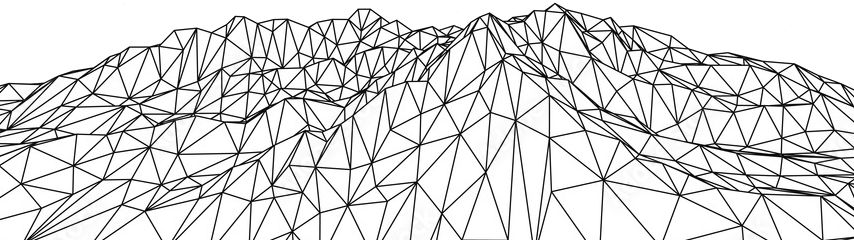
\includegraphics[width=\paperwidth]{../Unidad 2/Images/cover_bg}
\end{document}

\restoregeometry
\addtocontents{toc}{\setcounter{tocdepth}{3}}
\tableofcontents
\newpage
\chapter{}
\pagestyle{fancy}
\newpage
\thispagestyle{empty}
\section{Fracciones y decimales}
\subsection{Equivalencias de fracciones y decimales}
\subsection{Decimales peri\'odicos}
\subsubsection{Redondeo y truncamiento}

\newpage \thispagestyle{plain}

\section{Recta Num\'erica, Densidad y Orden}
\subsection{Fracciones en la Recta Num\'erica, Densidad y Orden}
\subsection{Decimales en la Recta Num\'erica, Densidad y Orden}
\subsection{Orden de fracciones y decimales}
\subsubsection{Orden en los n\'umeros fraccionarios}
\subsubsection{Orden en los n\'umeros decimales}


\newpage \thispagestyle{plain}
\section{Problemas con sumas y restas}
\subsection{N\'umeros con signo, recta y orden}
\subsection{Suma y resta de n\'umeros con signo}
\subsubsection{Suma de numeros con signo}
\subsubsection{Conmutatividad aditiva}
\subsubsection{Resta de n\'umeros con signo}
\newpage \thispagestyle{plain}
\section{Multiplicaci\'on con n\'umeros fraccionarios y decimales}
\subsection{Multiplicaci\'on con n\'umeros fraccionarios}
\subsection{Multiplicaci\'on con n\'umeros decimales}
\newpage \thispagestyle{plain}
\section{Divisi\'on con n\'umeros fraccionarios y decimales}
\newpage \thispagestyle{plain}
\section{\'Angulos, tri\'angulos y cuadril\'ateros}
\subsection{\'Angulos y rectas paralelas}
\subsection{Suma de los \'angulos interiores de un tri\'angulo y de un cuadril\'atero}
\subsubsection{\'Angulos de un tri\'angulo}
\subsubsection{\'Angulos de un cuadril\'atero}
\newpage \thispagestyle{plain}
\section{Tri\'angulos, cuadril\'ateros y congruencia}
\subsection{Criterios de congruencia}

\newpage \thispagestyle{plain}
\chapter{}
\newpage \thispagestyle{plain}
\section{Jerarqu\'ia de operaciones y signos de agrupaci\'on}
\boxabstract{
  Determina y usa la jerarquía de operaciones y los paréntesis en operaciones con números naturales, enteros y
  decimales (para multiplicación y división, sólo números positivos).
}

\subsection{Jerarqu\'ia de operaciones y signos de agrupaci\'on}
Dentro de las operaciones básicas de la aritmética existe una \textbf{jerarquía de operaciones}, es decir un
\textbf{orden}.

Recuerda cuando estabas en primaria y empezabas a leer, ¿qué aprendiste primero? Seguro fueron las vocales,
después fueron sílabas, después palabras completas hasta poder llegar a los enunciados y dentro de los enunciados
vienen los signos de puntuación, las comas, los dos puntos, el punto y seguido, el punto aparte, etc. Y entendiste la importancia de los signos de puntuación.

En los siguientes enunciados podemos observar ejemplos:
\begin{center}
  \begin{minipage}{0.4\textwidth}
    \begin{bA}
      Perdón imposible, castigarlo.\\
      Perdón, imposible castigarlo.
    \end{bA}
  \end{minipage}
\end{center}

Como podemos ver el significado de ambas expresiones son diferentes, bueno de eso se trata, en las matemáticas
existen reglas que si no se siguen el resultado de la operación sería incorrecto.

La operación de suma, resta, multiplicación y división tienen el siguiente orden:
\begin{figure}[H]
  \centering
  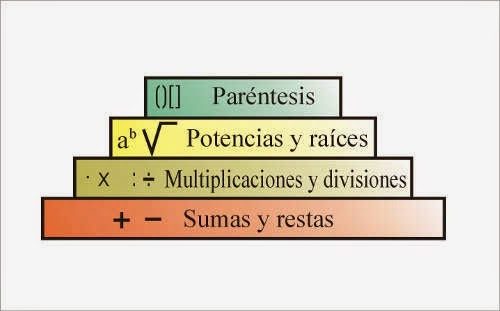
\includegraphics[width=0.5\textwidth]{./Unidad 2/Images/jerarquia.jpg}
\end{figure}

\subsubsection{Ejemplo 1: En este ejercicio haremos uso del paréntesis}

\[( 10 + 2 ) / 3 - 2\]

Observemos en este primer ejemplo se tiene un paréntesis y tiene mayor jerarquía, por lo que primero se realiza
esta operación.

\[12 / 3 - 2\]

Seguimos con el operador que tiene la jerarquía mas alta que es la división, y vamos de izquierda a derecha y
realizamos la operación.

\[4 - 2\]

Y por último, al resultado se le restan 2. Por lo que la operación nos queda:

\[( 10 + 2 ) / 3 - 2 = 2\]



\subsubsection{Ejemplo 2: En este ejercicio no utilizaremos el paréntesis}


Ahora vamos a ver el mismo problema pero sin el paréntesis.

\[5 + 6 / 2 - 2\]

Observemos que ahora la jerarquía mas alta la tiene primero la división, ya que no existe ningún paréntesis.

\[8 + 2 - 2 = 8\]

Vamos de izquierda a derecha, hacemos primero la suma y luego la resta y tenemos el resultado, como podemos apreciar
la gran importancia de respetar el orden de las operaciones para poder encontrar el resultado correcto.


\subsubsection{Ejemplo 3: En este ejercicio explicaremos un poco más detallado}

\[4 - 6 / 2 + 5 \times 2\]

Vamos de izquierda a derecha y hacemos la división por que en este ejemplo es el operador con mas jerarquía.

\[4 - 3 + 5 \times 2\]

Luego vamos de izquierda a derecha buscando el operador que tiene la mayor jerarquía para hacer la operaci\'on.
El cual es la multiplicaciónn.

\[4 - 3 + 10\]

Seguimos con la resta por izquierda y luego por la derecha

\[1 + 10\]

Por ultimo el resultado es el número 11.

\[4 - 6 / 2 + 5 \times 2 = 11\]

\newpage \thispagestyle{plain}
\section{Resolución de problemas con valores faltantes}
\boxabstract{Calcula valores faltantes en problemas de proporcionalidad directa,
  con constante natural, fracción o decimal (incluyendo tablas de variación).}

\subsection{Proporcionalidad directa y valor faltante}
\begin{boxK}
  \begin{center}\textbf{Inicio}\end{center}
  Menhir el arquitecto hizo un obelisco para conmemorar los setenta y seis años de su padre.
  Ahora hace un obelisco de menor tamaño, pero con la misma forma y del mismo material
  que el de su padre, para celebrar el decimonoveno cumpleaños de su hijo.
  \begin{enumerate}
    \item Las medidas de los obeliscos de Menhir están en la misma proporción que hay entre las
          edades de su padre y de su hijo. Si la altura del obelisco hecho en honor al padre es de
          12.2 m, ¿qué altura tiene el obelisco dedicado al hijo?

    \item Los obeliscos tienen base cuadrada. Si la base del obelisco dedicado al hijo tiene una
          longitud de 0.80 m por lado, ¿cuánto mide el lado de la base del obelisco más grande?
    \item Compartan sus respuestas y procedimientos con sus compañeros y escriban en su cua-
          derno el procedimiento que les parezca más acertado.
  \end{enumerate}
\end{boxK}

\begin{enumerate}
  \item En el local de jugos de Ana para preparar dos litros de agua de frutas se agregan,
        además de las frutas, cinco cucharadas de azúcar. Contesta lo siguiente
        \begin{enumerate}
          \item Si se mantiene la misma proporción, ¿cuántas cucharadas se necesitan para preparar ocho litros?
          \item Si agregó 33 cucharadas, ¿cuántos litros preparó?
          \item Si Ana utilizó 15 cucharadas, ¿cuántos litros prepararó?
          \item ¿Cuántas cucharadas se requieren para preparar un litro de agua?
        \end{enumerate}
  \item  Para llenar un vitrolero se necesitan cuatro litros de agua. Completa la tabla para
        saber cuántas cucharadas necesita Ana.
        \begin{figure}[H]
          \centering
          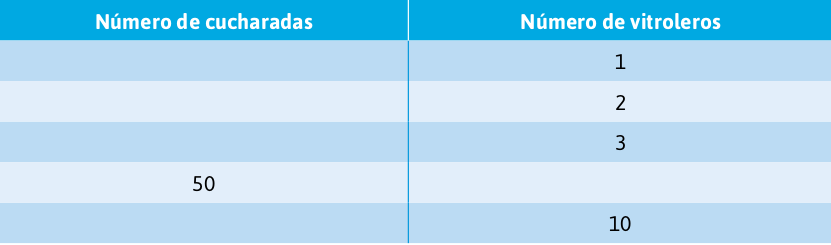
\includegraphics[width=0.6\linewidth]{tabla_vitrolero.png}
          \captionof{table}{}
          \label{tab:tabla_vitrolero}
        \end{figure}
        \begin{enumerate}
          \item ¿Cuántas cucharadas se necesitan para preparar un vitrolero?
          \item Si el número de vitroleros aumenta al doble, ¿cómo se incrementa el número de
                cucharadas? ¿Y si aumenta al triple?
          \item Explica en tu cuaderno, cómo determinarías el número de cucharadas a partir del
                número de vitroleros.
        \end{enumerate}

  \item Durante el Renacimiento, el estudio de la anatomía humana tuvo gran auge. Uno
        de los trabajos más conocidos es \emph{El hombre de Vitrubio} (ver figura \ref{fig:Hombre-de-Vitruvio}) de Leonardo
        da Vinci. Una de las proporciones más interesantes en esta obra es la relación entre
        la estatura de la figura y la distancia entre el ombligo y la base de los pies.

        \begin{minipage}{0.45\textwidth}
          \begin{figure}[H]
            \centering
            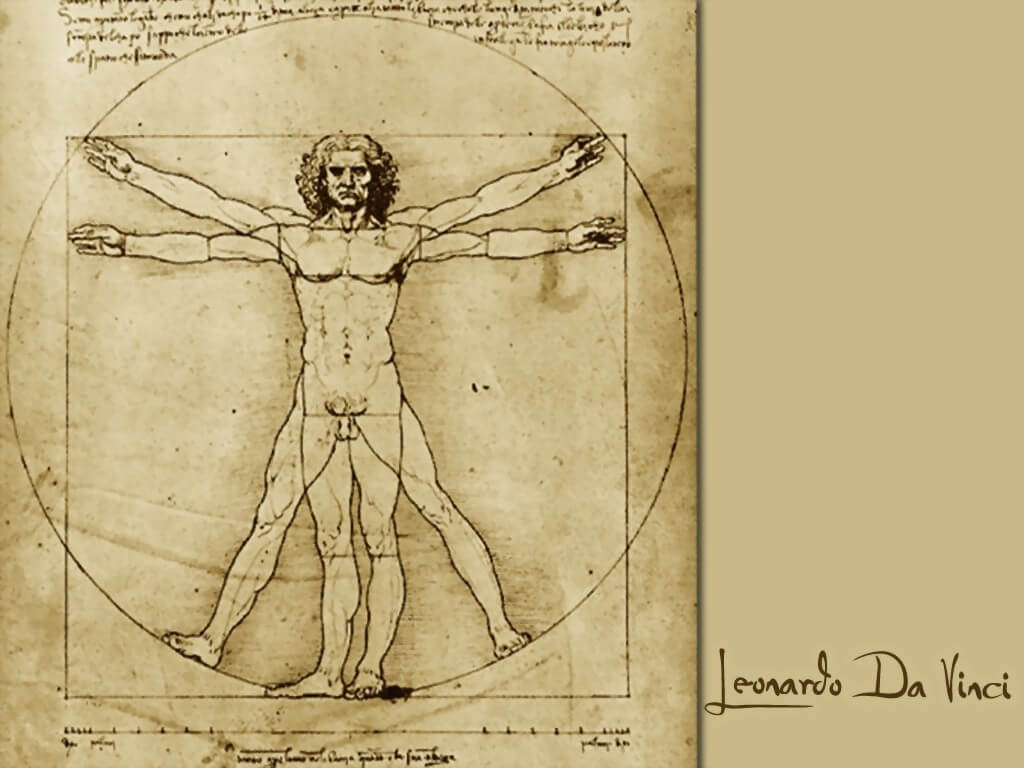
\includegraphics[width=\linewidth]{Hombre-de-Vitruvio.jpg}
            \captionof{figure}{Obra de Leonardo Da Vinci, titulada \emph{El hombre de Vitrubio}}
            \label{fig:Hombre-de-Vitruvio}
          \end{figure}
        \end{minipage}\hfill
        \begin{minipage}{0.45\textwidth}
          \begin{boxH}
            Dos magnitudes tienen una relación de proporcionalidad directa si al aumentar o
            disminuir una la otra aumenta o disminuye, respectivamente, en la misma proporción.
            En este caso, al calcular la razón entre un valor de la primera magnitud y su correspondiente
            de la otra magnitud, siempre obtendremos un número constante.
            Si en una relación de proporcionalidad directa se desconoce un valor, se dice que
            se trata de un problema de valor faltante.
          \end{boxH}

        \end{minipage}
        \begin{boxE}
          En \emph{El hombre de Vitrubio} se dice que la razón de su estatura respecto a la distancia
          del ombligo a los pies es perfecta y su valor es un número decimal no periódico e
          infinito: 1.61803\dots llamado \emph{proporción aúrea} (que redondeamos a 1.62).
        \end{boxE}

        \begin{enumerate}
          \begin{figure}[H]
            \centering
            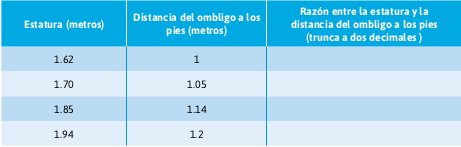
\includegraphics[width=0.6\linewidth]{tabla_hombre.png}
          \end{figure}
          \item Completa la tabla que relaciona la estatura de cuatro personas y la distancia de
                su ombligo a sus pies.
          \item ¿Qué observas en la última columna?

        \end{enumerate}

\end{enumerate}

\begin{boxK}
  \begin{center}\textbf{Cierre}\end{center}
  Regresa al problema inicial, identifica una relación de proporcionalidad directa y calcula
  la constante de proporcionalidad.
  Revisa tus respuestas a los incisos $a$ y $b$ y valida el procedimiento del inciso $c$.
\end{boxK}

\subsection{Proporcionalidad y valor unitario}

\begin{boxK}
  \begin{center}\textbf{Inicio}\end{center}
  Manolo y Sebastián compraron una bolsa con 100 canicas como la que se muestra en la
  figura, por \$80.00. Manolo aportó \$32.00 y Sebastián completó el pago.
  \begin{enumerate}
    \item ¿Cuánto pagó Sebastián?
    \item ¿Te parece justo que, al repartirlas, cada uno tenga 50 canicas? ¿Por qué?
    \item ¿Cuántas canicas debería recibir cada uno de acuerdo con lo que aportaron?
    \item Explica cómo decidiste repartir las canicas entre Manolo y Sebastián, y por qué
          consideras que de esa manera el reparto es justo.
  \end{enumerate}
\end{boxK}

\begin{minipage}[t]{0.2\textwidth}
  \begin{figure}[H]
    \centering
    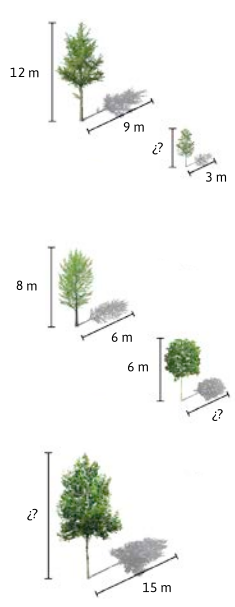
\includegraphics[width=1.4\linewidth]{fig_sombras.png}
    \captionof{figure}{}
    \label{fig:fig_sombras}
  \end{figure}
\end{minipage}\hfill
\begin{minipage}[t]{0.75\textwidth}
  \begin{enumerate}
    \item En un día soleado los objetos forman sombras y, a la misma hora, la altura y la
          sombra de diferentes objetos es proporcional.
          \begin{flushright}
            \begin{figure}[H]
              \centering
              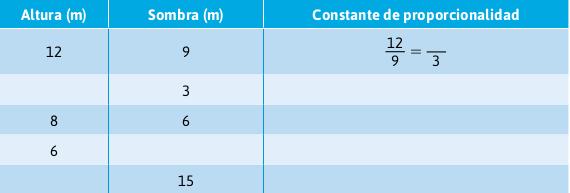
\includegraphics[width=0.85\linewidth]{tabla_sombras.png}
              \captionof{table}{}
              \label{tab:tabla_sombras}
            \end{figure}
          \end{flushright}
          \begin{enumerate}
            \item Con la información de la figura completa la tabla \ref{tab:tabla_sombras}.
            \item ¿Cómo son los números de la última columna?
            \item Si la sombra de un árbol mide 7.5 m, ¿cómo calcularías su altura? Explica.
            \item  En primaria aprendiste a ubicar puntos en el plano cartesiano por medio de
                  coordenadas. Ubica los puntos cuyas coordenadas corresponden a la altura y sombra de los árboles
          \end{enumerate}
  \end{enumerate}
\end{minipage}
\newpage
\begin{figure}[H]
  \centering
  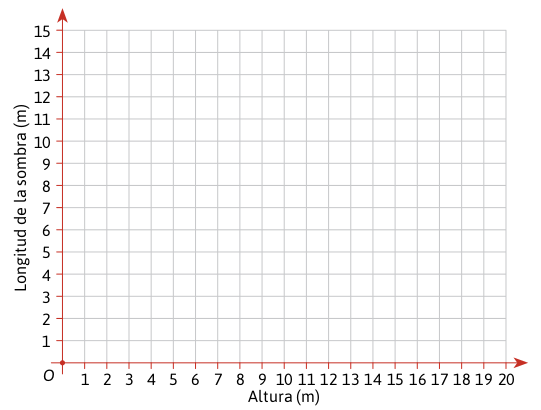
\includegraphics[width=.75\linewidth]{plano_sombras.png}
\end{figure}

\newpage

\subsection{Resolución de problemas de proporcionalidad directa}

\newpage \thispagestyle{plain}
\section{Porcentajes}
\boxabstract{Resuelve problemas de cálculo de porcentajes, de tanto por ciento y de la cantidad base.}

\subsection{Tanto por ciento}
\subsection{Cálculo del porcentaje}
\subsection{Porcentajes y aplicaciones}

\newpage \thispagestyle{plain}
\section{Perímetros y áreas}
\boxabstract{Calcula el perímetro de polígonos y del círculo, y áreas de triángulos y cuadriláteros desarrollando
  y aplicando fórmulas.}
\subsection{Perímetro de polígonos}
\subsection{Perímetro del círculo}
\subsection{Áreas de triángulos y cuadriláteros}
\newpage \thispagestyle{plain}
\section{Ecuaciones lineales}
\boxabstract{Resuelve problemas mediante la formulación y solución algebraica de ecuaciones lineales.}
\subsection{Formulación de ecuaciones}
\subsection{Solución de una ecuación}




\newpage \thispagestyle{plain}
\section{Resolución de ecuaciones lineales}
\boxabstract{Resuelve problemas mediante la formulación y solución algebraica de ecuaciones lineales.}
\subsection{Propiedades de la igualdad}
\subsection{Más sobre ecuaciones lineales}






\newpage \thispagestyle{plain}
\section{Medidas de tendencia central}
\boxabstract{Usa e interpreta las medidas de tendencia central (moda, media aritmética y mediana) y el
  rango de un conjunto de datos, y decide cuál de ellas conviene más en el análisis de los datos en cuestión.}
\subsection{Media aritmética o promedio}
\subsection{La media aritmética y el rango}





\newpage \thispagestyle{plain}
\section{Moda, media aritmética y mediana}
\boxabstract{Usa e interpreta las medidas de tendencia central (moda, media aritmética y mediana) y
  el rango de un conjunto de datos, y decide cuál de ellas conviene más en el análisis de los datos en cuestión.
}
\subsection{Media aritmética y mediana}
\subsection{Moda}
\subsection{Representantes de un grupo de datos}

\chapter{}

\section{Situaciones de variación proporcional}
\subsection{Comparación de situaciones de variación proporcional con tablas}
\subsection{Comparación de situaciones de variación proporcional con gráficas}
\subsection{Comparación de situaciones de variación proporcional con expresiones algebraicas}




\newpage \thispagestyle{plain}
\section{Pendiente de una recta y razón de cambio}
\subsection{Variación proporcional y pendiente}
\subsection{Razón de cambio y variación}
\subsection{Efectos en la recta al cambiar la pendiente}

\newpage \thispagestyle{plain}
\section{Análisis y comparación de situaciones de variación lineal}
\subsection{Efectos de la recta al cambiar la ordenada al origen}
\subsection{Situaciones de variación lineal asociadas a la física, la biología y la economía}

\newpage \thispagestyle{plain}
\section{Sucesiones y expresiones algebraicas}
\subsection{Sucesiones numéricas}
\subsection{Sucesiones con progresión aritmética}

\newpage \thispagestyle{plain}
\section{Congruencia de triángulos y aplicaciones}
\subsection{Aplicaciones de congruencia de triángulos}
\subsection{Aplicaciones a cuadriláteros}

\newpage \thispagestyle{plain}
\section{Vol\'umenes de prismas rectos}
\subsection{Volumen de prismas rectos rectangulares}
\subsection{Fórmula del volumen de prismas rectos}

\newpage \thispagestyle{plain}
\section{Gráficas circulares}
\subsection{Recolecta y registra datos}
\subsection{Registra datos en gráficas circulares}
\subsection{Leer e interpretar datos en gráficas circulares}

\newpage \thispagestyle{plain}
\section{El azar y la probabilidad frecuencial}
\subsection{Tipos, recolección y organización de datos}
\subsection{Experimentos aleatorios y deterministas}
\subsection{Espacio muestral de un experimento aleatorio}
\subsection{Cálculo de la probabilidad frecuencial}


\end{document}





